\chapter{背景:音楽}

本章では、本論文での音の定義を行った後に、音楽の特徴量抽出の方法を紹介する。

\section{音の定義}

音とは、弾性体中を伝播する弾性波により起こされる音波が聴覚により感じられるもののことである。また、音は騒音と楽音の大きく二つに分けることができる。騒音とは不規則な振動の音波による音のことであり、楽音とは周期生のある音波による音のことである。本論文では、楽音のことを音と呼ぶ。

音は長さ、大きさ、高さ、音色の四要素から成り立ち、人間はこれらの要素を知覚することができる。また、図\ref{fig:gakuon}は音の四要素について簡単に示した図である。

\begin{figure}[b]
\begin{center}
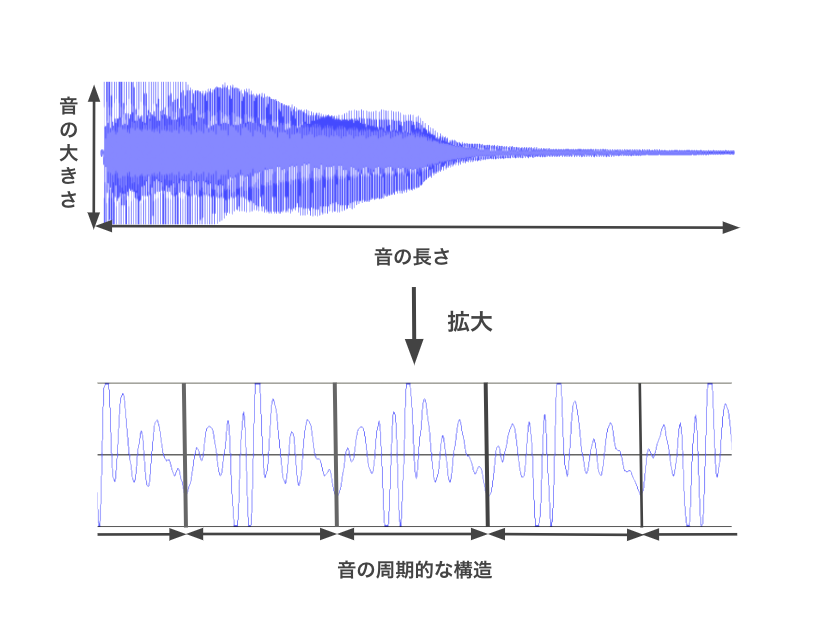
\includegraphics[width=0.6\hsize]{figure/gakuon.png}
\caption{音の四要素}
\label{fig:gakuon}
\end{center}
\end{figure}

\subsection{音の長さ}

音の長さは図\ref{fig:gakuon}のように音波の時間の長さにより決まる。一般に、音の長さは楽譜上での時間の長さ~(音価)~により決まるが、本論文では音波の時間の長さにより決まるものとする。

\subsection{音の大きさ}

音の大きさは図\ref{fig:gakuon}のように音波の振幅により決まる。また、人間には振幅の大きい音は大きく、振幅の小さい音は小さく知覚される。

\subsection{音の高さ}

音の高さは音波の周波数により決まる。つまり、図\ref{fig:gakuon}のような音の周期的な構造の長さにより決まる。また、人間には周波数の高い音は高く、周波数の低い音は低く知覚さる。そして、複数の周波数の音波が音に含まれる場合は最も低い周波数成分の音波~(基音)~を音の高さとして知覚する。

国際の音名表記では、C,D,E,F,G,A,Bのセットを西洋音楽の七音音階におけるオクターブとして定める。さらに、それぞれのオクターブに番号を振り、440~Hzの音をA4と定めることで、任意の半音の絶対的な表記を可能にしている。また、国際の音名表記では半音よりさらに細かい音~(微分音)~を表すことはできないが、本論文では扱わない。

\subsection{音の音色}

音の長さと高さと大きさが同じであっても異なった音として人間には知覚されることがある。この違いを音色と呼ぶ。また、音色は図\ref{fig:gakuon}のような音の周期的な構造の形により決まる。

\begin{figure}[b]
\begin{center}
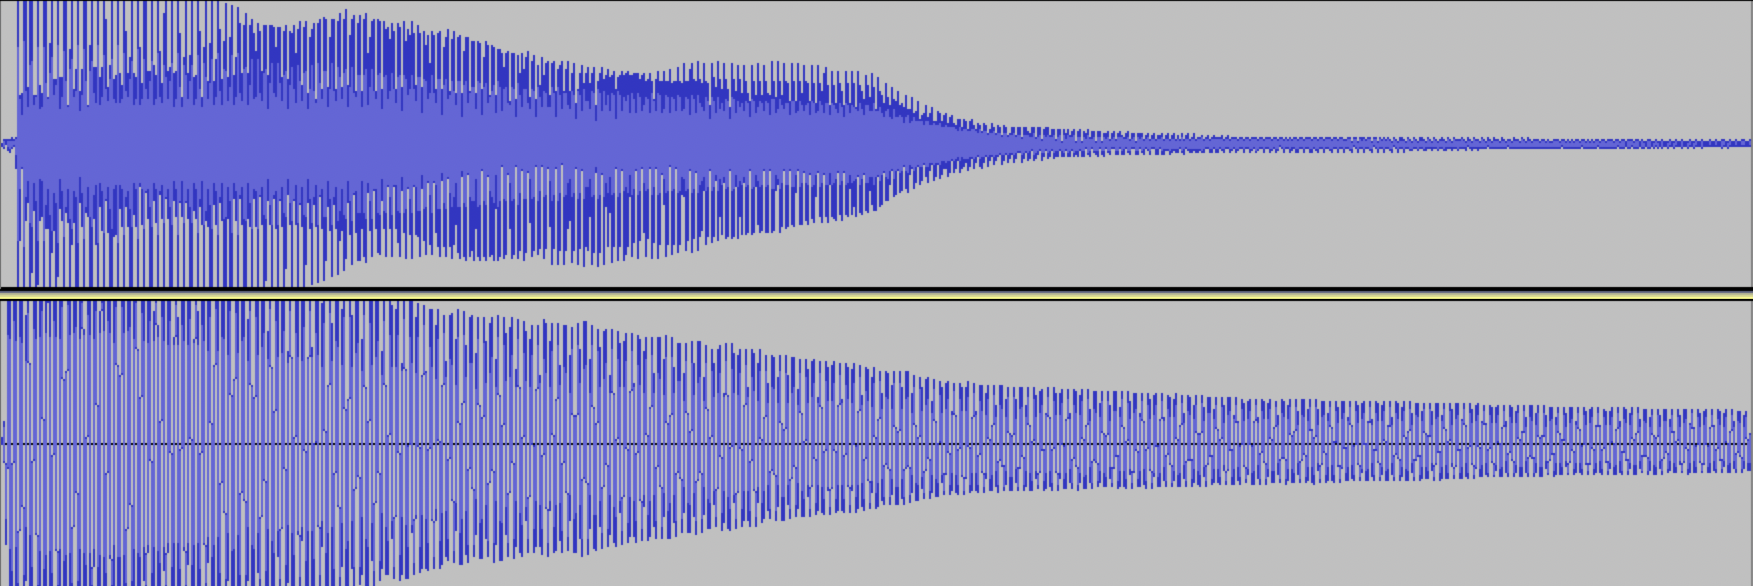
\includegraphics[width=\hsize]{figure/c4_guitar_harp.png}
\caption{ギターとハープの音色}
\label{fig:guitar_harp_comp}
\end{center}
\end{figure}

ここで、長さと高さと大きさが同じギターとハープの音波を図\ref{fig:guitar_harp_comp}に示す。これらの音は波形が異なるので、その音色も異なる。また、音色の異なる音どうしは基音よりも高い音~(上音)~の組み合わせが異なるため、このような波形の違いが生まれる。

\section{音楽の特徴}

%以下の自分の考えと融合させる
\begin{comment}
\section{展望}

一般に、音楽で特定の音色への変換を行うことは難しいが、次の三つの要素に分解することで単音での音色の変換を音楽へと適用することが可能であると考えられる。また、三つの要素とは、楽器の重ね合わせ、音の重ね合わせ、時間方向の音の繋ぎ方であり、それぞれについて具体的に以下で説明をする。

\subsection{楽器の重ね合わせ}
    
音楽はそれぞれの楽器により奏でられた音の重ね合わせになっている。楽器ごとに音色は異なるので楽器ごとの音波に分解して音色変換を行う~(音源分離)~が必要であると考えられる。なお、楽曲の作成時に楽器ごとに分離したデータ~(パラデータ)~で保存しておけば、音源分離を行わずに直接楽器ごとの音波を利用できる。

\subsection{音の重ね合わせ}

ある単位時間の音に注目した時、楽器ごとの音波に分解してもその単位時間で異なった高さや大きさの音の重ね合わせになっていることがある。この場合は、今回の提案手法で用意したデータセット以外に和音のデータセットも加えて学習させることで表現可能であると考えられる。

\subsection{音の繋ぎ方}

%他の工夫があるかも

楽器ごとの音波に分解し単位時間の音が表現できた時、時間方向に音を繋ぐ必要がある。時間方向については先程定めた単位時間で区切って順に変換していくことで可能であると 考えている。また、区切るのみでの変換が難しい場合は自己回帰モデルを取り入れるなどの工夫が必要であると考えている。
\end{comment}

音楽をニューラルネットワークにて扱う場合、音楽特有の特徴量抽出が必要である。また、音楽の特徴には、主観的な問題とタイムスケールの問題がある。

\subsection{音楽の主観性}

まず、主観性について。例えば、音楽のジャンルの分け方はかなり主観に依存する。それに対し、ピッチやテンポは主観性が弱い(が、曖昧でもある)。ディープラーニングはこれらの二つの問題に対してある程度対応できている。主観さの裏にある論理を解明しない限りは、人間の手で特徴量を設定するのは難しい。従って、データ駆動でend-to-endな学習を利用することができる。さらに、新たな洞察を得ることもできる。例えば、異なる音楽間の関係性。また、よく知られた論理があればネットワーク構築にも役立つ。

\subsection{音楽の時間方向のスケール}

次にタイムスケールについて、考慮すべき時間のスケール。例えば、テンポや音の高さは音楽全体では変化するものの短い時間で見れば静的である。このような場合は時間のスケールは長いと言える(時間不変性の問題)。それに対し、音色は短いスケールのタイムフレームであっても変わりうる。従って、このような場合は時間のスケールは短い(時間可変性の問題)。

このように、それぞれの特徴が異なった主観性やタイムスケールを持つので、対処法が変わってしまう。

% 以降は式を含めて詳しく書く(ちゃんと勉強してから)
% 具体例もある程度読む(自分の読んだやつの方が良いかも)、DDSPも

\section{音楽の表現}
\label{sec:preprocess}

%既存研究の紹介、単語の説明、もう少し短く

ニューラルネットワークで音楽を扱うためには表現の工夫が必要である。まず、基本的な表現は一次元データの音響信号であるが、ほとんどの場合は何らかの加工を施した二次元データである。また、二次元の軸としては周波数と時間を選ぶことが多い。この時、音楽のどのような特徴を把握したいか及びネットワークの時間計算量と空間計算量に合わせて適切な表現を選ぶ必要がある。

そして、多くの場合、二次元データでは中心周波数を利用したフィルタを用いて音響信号を分解し、信号を明確化する。これにより、効果的なデータ表現として扱うことができる。さらに、二次元の場合は画像と同じアルゴリズムを用いることができるが、異なる特徴が存在する。まず、画像の場合は局所的な相互関係が存在する。例えば、近くのピクセル同士は色合いや強度が似ている。しかし、スペクトログラムでは、周波数成分の方向で調和的な関係は存在する一方で局所的な相互関係は弱い。また、調和的な関係を把握するために表現を変更するような研究もある。そして、物体認識ではスケール不変性も求められるが、音楽についてはあまり関係はないと考えられる。

\subsection{音響信号}

%既存研究の紹介

音響信号とは信号としての音の呼び名である。また、連続量である音響信号~(アナログ信号)~はコンピュータではデジタル信号に変換されて処理される。この時、標本化~(サンプリング)~と量子化が必要である。サンプリングとはアナログ信号を一定の間隔を空けて離散的に測定を行うことであり、量子化とは信号の大きさを離散的に近似して表現することである。そして、1秒あたりのサンプリング回数をサンプリング周波数、信号の大きさを表現するビット数を量子化ビット数、と呼ぶ。

音響信号は一次元の音の素朴な表現であるが、ニューラルネットワークの学習により音の特徴を把握するには多くのデータセットが必要になると考えられ、以降で紹介する二次元での表現へと変換されて扱われることが多い。ただ、〇〇などの研究では音響信号のままニューラルネットワークを用いることがあり、本研究ではこちらの音響信号の形で音を扱った。

\subsection{STFT}

STFTは線形間隔の中心周波数を用いて周波数成分を分解し、時間-周波数の二次元の表現を行う方法である。また、高速フーリエ変換を用いることにより、他の二次元の表現と比べて高速に計算を行うことができる。

しかし、線形間隔の中心周波数の利用は音楽に適しているとは言えない。なぜなら、人間の知覚系の周波数分解能は線形とかなり異なるからである。また、STFTは音楽の解析のために作られたわけでもないからである。これらの理由から、STFTはディープラーニングにおいては最も人気のある手法ではない。

ただし、STFTの音響信号との間の可逆性を利用して、音源分離などに用いられる。

\subsection{メルスペクトログラム}

メルスペクトログラムは人間の知覚系に合わせて最適化された二次元の表現であ李、STFTにおいて周波数方向に関してメル尺度~\cite{melscale}を用いて圧縮を行ったものである。そのため、知覚として必要な情報を保持したまま圧縮を行うことができる。ただし、メルスペクトログラムは位相の情報を保持せず音の大きさのみを保持しているため、音響信号との間で非可逆的である。

また、メル尺度を表す式にはいくつかあり、式\ref{eq:mel}はその一つである。

\begin{align}
    \label{eq:mel}
\end{align}

経験的かつ心理的な理由でメル尺度を用いたメルスペクトログラムは音楽のタスクに適している。(例もある)

\subsection{CQT}

CQTは対数振幅の中心周波数を使用した二次元の表現である。CQTは対数振幅を用いており、音の高さの分布に近い。したがって、基音を正確に識別する際に用いられ、和音の識別や書き換えに使うことができる。

また、計算量としてはSTFTやメルスペクトログラムより重い。そして、単純な対数振幅のスペクトログラムが有効な例もある。

\subsection{クロマグラム}

与えられた音の高さの集合におけるエネルギー分布のこと。多くの場合は西洋音楽の12音階をその集合とする。つまり、クロマグラムは周波数方向に畳み込んだCQTと見なすことができる。また、クロマグラムは他の表現方法よりも処理が進んだものなので、それ自身を特徴量として用いることができる。
